\documentclass[11pt,letterpaper]{article}
\usepackage[T1]{fontenc}
\usepackage{fullpage}
\usepackage[top=2cm, bottom=4.5cm, left=2.5cm, right=2.5cm]{geometry}
\usepackage{amsmath,amsfonts,amssymb}
\usepackage{lastpage}
\usepackage[inline]{enumitem}
\usepackage{fancyhdr}
\usepackage{mathrsfs}
\usepackage{xcolor}
\usepackage{graphicx}
\usepackage{subcaption}
\usepackage{appendix}
\usepackage{hyperref}
\usepackage{titlesec}
\usepackage{fancyvrb}
\hypersetup{colorlinks=true, linkcolor=blue, linkbordercolor={0 0 1}}

%\renewcommand{\arraystretch}{1.5}
\titlespacing*{\section}{0pt}{0.65\baselineskip}{0.5\baselineskip}

\setlength{\parindent}{0.0in}
\setlength{\parskip}{0.05in}

\newcommand{\qrf}{\texttt{QRFactor}}

\pagestyle{fancyplain}
\lhead{}
\chead{GPU Solutions for PSCAD: IT17112}
\rhead{}
\cfoot{\small\thepage}
\headsep 32pt

%%%%%%%%%%%%%%%%%%%%%%%%%%%%%%%%%%%%%%%%%%%%%%%%%%%%%%%%%%%%%%%%%%%%%%%%%%%%%%%
%%%%%%%%%%%%%%%%%%%%%%%%%%%%%%%%%%%%%%%%%%%%%%%%%%%%%%%%%%%%%%%%%%%%%%%%%%%%%%%

\begin{document}
\begin{center}
    {\Large \bf Monthly Summary: September, 2020}
\end{center}

The primary goal of the work this month was the development of an interface between existing PSCAD code and \verb+QRFactor+. This process required a fundamental shift in the implementation of \verb+QRFactor+ from the standard, single-file CUDA project to a more object-oriented approach. This way, the system matrix could be factored and held on the device as its own object while repeated calls with some right hand side vector $\mathbf{b}$ as an input would return the desired output $\mathbf{x}$ from the equation $A\mathbf{x} = \mathbf{b}$. This would mean that the class QRFactor would need to support device-side functions as well as host-side functions. In this summary, we discuss the structure of our object-oriented approach as well as the technical details that need to be addressed to include GPU code within a standard C++ program.

%%%%%%%%%%%%%%%%%%%%%%%%%%%%%%%%%%%%%%%%%%%%%%%%%%%%%%%%%%%%%%%%%%%%%%%%%%%%%%%

\section*{The QRFactor Class}

The QRFactor class provides the required interface between the existing PSCAD program and the GPU-based methods incorporated into \qrf. In figure~\ref{f:qrclass}, we present a schematic of the structure of this class. 

\begin{figure}[ht]
    \centering
    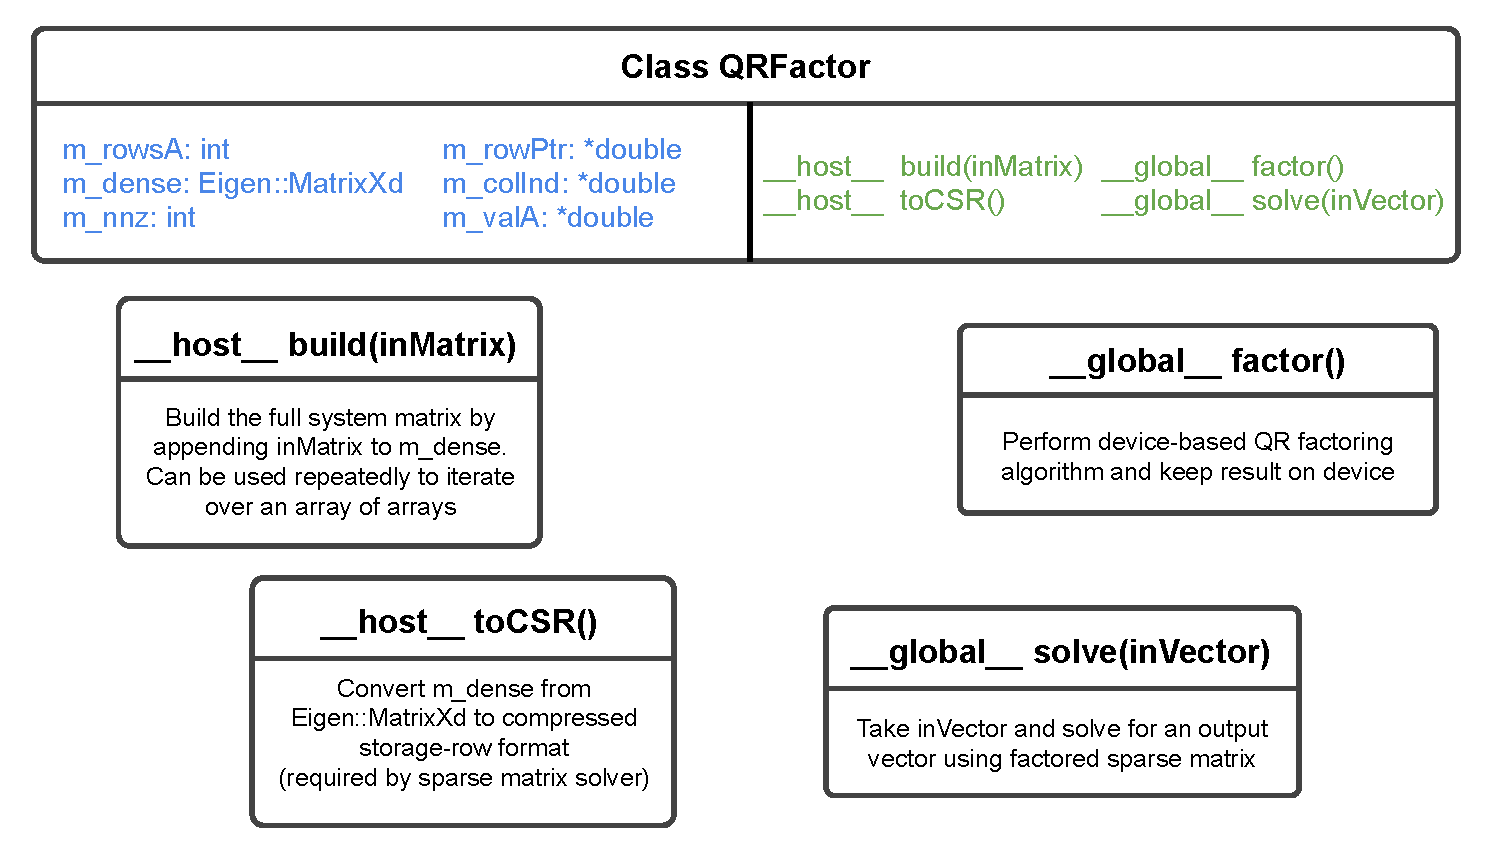
\includegraphics[width=0.75\textwidth]{MHI QRFactor.pdf}
    \caption{{\it Schematic of the QRFactor class. Class variables are shown in blue while class functions are shown in green.}}
    \label{f:qrclass}
\end{figure}

In the event that GPU methods are required for a particular problem, the existing PSCAD code will pass an array of dense matrices to \verb+QRFactor+. These dense matrices must be assembled into a single, large (sparse) system matrix before being passed to the GPU for factoring. To achieve this, the QRFactor class has a private dense matrix \verb+m_dense+ that can be iteratively extended to include the smaller submatrices. This occurs on the CPU with the open source \href{http://eigen.tuxfamily.org/index.php?title=Main_Page}{Eigen package}, an optimized C++ library for manipulating and solving linear systems. Once all the subsystems have been combined to give the full system matrix, another CPU function will convert the matrix into the compressed storage format that is required for factoring and solving on the GPU. 

The device-side functions \verb+factor+ and \verb+solve+ perform the factoring of the system matrix $A$ into $QR$ and the solve for $\mathbf{x}$ given an input $\mathbf{b}$. These function in the same way as the stand-alone \verb+QRFactor+ program. Along with the class functions shown in figure~\ref{f:qrclass}, there are also several small \verb+get+ and \verb+set+ functions for the private class variables. Finally, to ease in later debugging, the QRFactor class has its own set of error codes that describe where in the build, conversion, factoring, or solving processes an error occurs.

%%%%%%%%%%%%%%%%%%%%%%%%%%%%%%%%%%%%%%%%%%%%%%%%%%%%%%%%%%%%%%%%%%%%%%%%%%%%%%%

\section*{Compiling \& Linking}

Unlike the previous versions of \verb+QRFactor+, the new interface requires the separate compilation of source files that contained a mix of CPU and GPU functions. In order to achieve this, the NVIDIA compiler \verb+nvcc+ must compile .cpp files as .cu files if CUDA code was detected, but pass .cpp files \emph{without} CUDA code to the standard compiler. Furthermore, the NVIDIA linker needs to be able to link object files with device code to object files without device code to produce the final executable. To illustrate this process, we consider \href{https://developer.nvidia.com/blog/separate-compilation-linking-cuda-device-code/}{an example} of separate compilation and linking with mixed host and device functions that is available on the NVIDIA blog. See figure~\ref{f:example} for an illustration of the build structure for this example. 

\begin{figure}[h]
    \centering
    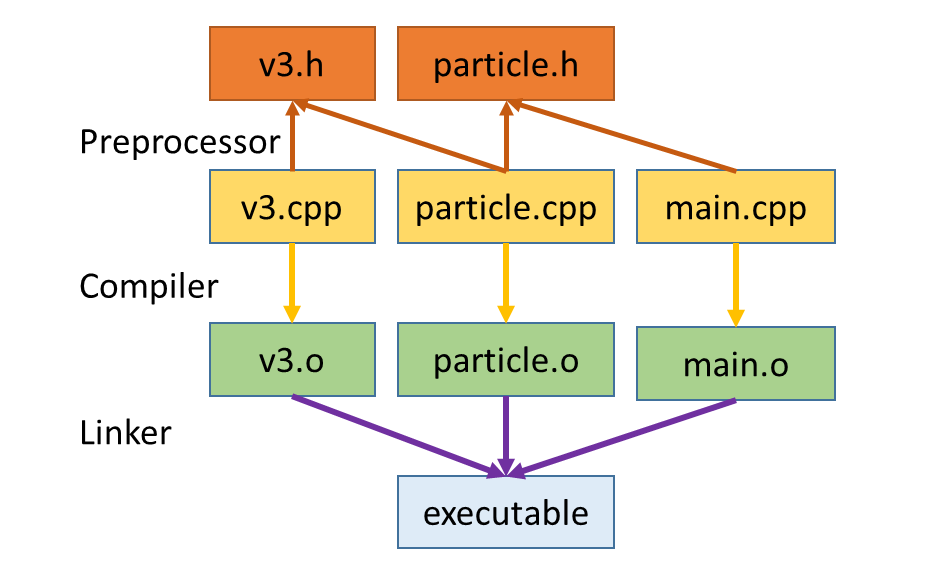
\includegraphics[width=0.75\textwidth]{C++BuildStructure.png}
    \caption[]{{\it C++ build structure for a sample program. Image credit \href{https://developer.nvidia.com/blog/separate-compilation-linking-cuda-device-code/}{NVIDIA blog}.}}
    \label{f:example}
\end{figure}

This example uses GPU-accelerated methods to describe the motion of a particle in three dimensions. The particle class contains functions that use both host-side functions and device-side functions, as well as relying on another class, v3, which itself contains mixed CPU and GPU functions. Like the functions that make up the QRFactor class, the \verb+__host__+, \verb+__device__+, and \verb+__global__+ decorators are used to indicate to the compiler whether to compile the functions as callable from the CPU only, the GPU only, or either. With these decorators written into the source files, calling \verb+nvcc+ with the \verb+-x cu+ option will tell the compiler to treat host code and device code differently, and the linker will be able to properly connect the resulting object files. In figure~\ref{f:makefile}, we see the \verb+-x+ flag being used during compilation. While the \qrf~interface is currently being developed in Microsoft Visual Studio 2019, similar calls to the compiler are encapsulated in the project settings for a CUDA Runtime template.

\begin{figure}[h]
    \centering
    \begin{tabular}{| p{0.45\textwidth} |}
        \hline
        objects = main.o particle.o v3.o \\
         \\
        all: \$(objects) \\
        $\quad$ nvcc -arch=sm\_20 \$(objects) -o app \\
         \\
        \%.o: \%.cpp \\
        $\quad$ nvcc -x cu -arch=sm\_20 -I. -dc  \$< -o  \$@ \\
         \\
        clean: \\
        $\quad$ rm -f *.o app \\ \hline
    \end{tabular}
    \caption{{\it The Makefile required to compile the sample program outlined in \ref{f:example}.}}
    \label{f:makefile}
\end{figure}

For additional comments on programs with separate compilation -- including possible options that can affect performance -- see Chapter 6 in the CUDA \href{https://docs.nvidia.com/cuda/pdf/CUDA_Compiler_Driver_NVCC.pdf}{NVCC Guide}.

The development of the \qrf~interface is ongoing but is nearing completion. Actual integration with PSCAD software is forthcoming, and there will be several factors to consider, including the possibility of a flag to avoid initial subsystem splitting if it can be determined that GPU-based methods will be superior to multicore CPU methods. It is hoped that these and other possible considerations should not require any significant rewriting of the \qrf~interface due to its object-oriented approach. 

%%%%%%%%%%%%%%%%%%%%%%%%%%%%%%%%%%%%%%%%%%%%%%%%%%%%%%%%%%%%%%%%%%%%%%%%%%%%%%%
%%%%%%%%%%%%%%%%%%%%%%%%%%%%%%%%%%%%%%%%%%%%%%%%%%%%%%%%%%%%%%%%%%%%%%%%%%%%%%%































\end{document}
